In order to make decisions based on images it is important to recognize objects.
Three image markers are given and the task is to find points that can represent the marker in the image.
In figure \ref{fig:markers} can the different markers be seen.
In the simulation, the ideal marker is used but the markers will be tested on a set of real images where lighting, rotation and translation makes the markers harder to detect.
The detector should evaluate the image and return whether the marker was found, and either the center of the marker or several fixed points on the marker.


\begin{figure}[h]
\centering
 \begin{subfigure}[b]{0.3\linewidth}
 \centering
 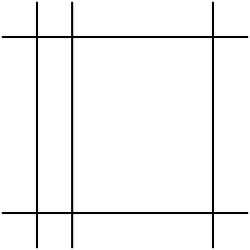
\includegraphics[width=\linewidth]{graphics/Marker2a}
 \caption{Crosses}
 \label{marker:cross}
 \end{subfigure}~
 \begin{subfigure}[b]{0.3\linewidth}
 \centering
 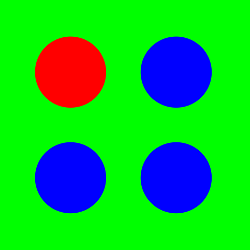
\includegraphics[width=\linewidth]{graphics/Marker1}
 \caption{Circles}
 \label{marker:circle}
 \end{subfigure}
 \begin{subfigure}[b]{0.3\linewidth}
 \centering
 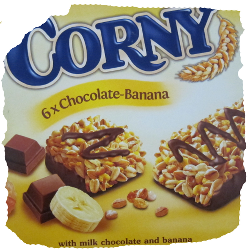
\includegraphics[width=\linewidth]{graphics/Marker3}
 \caption{Corny}
 \label{marker:corny}
 \end{subfigure}
 \caption{The different markers.}
 \label{fig:markers}
\end{figure}
